\section{Real-time Visualization} (0.5 page) (AJ, JP)
\label{sec:vis}

To enable our focus and context transparent visual, we require an ordered list of fragments for each screen pixel. This list of fragments is also commonly referred as an A-buffer. We implemented the A-buffer using per-pixel linked lists~\cite{yang2010real}. In our case, the A-buffer fragments represent three types of surface patches analytically computed for a given ray.

\subsection{Ray-casting}
\label{sec:spherical-patches}
To form fragments of each surface patch we employ a ray-casting technique. To provide a high performance, the ray-patch intersection is computed analytically.
In 2013, Kauker et al.~\cite{kauker2013rendering} proposed to ray-cast a toroidal patch using a torus and two clipping planes defined by its delimiting triangles (Fig.~\ref{fig:torus-vs}).
\begin{figure}[htp]
  \centering
  \begin{subfigure}[t]{0.55\columnwidth}
    \centering
    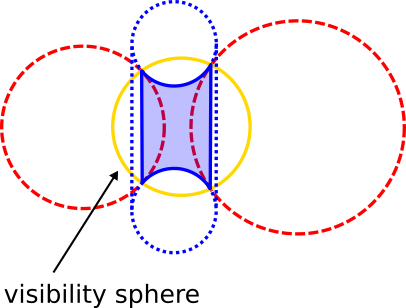
\includegraphics[width=1.7in]{image/torus-vs.png}
    \caption{Clipping by \textit{visibility sphere}.}
		\label{fig:torus-vs}
  \end{subfigure}%
  \quad
  \begin{subfigure}[t]{0.4\columnwidth}
    \centering
    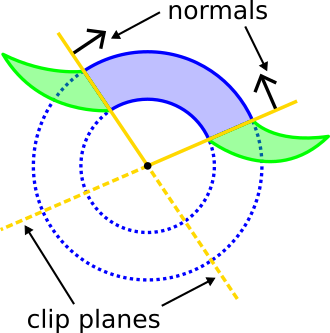
\includegraphics[width=1.3in]{image/torus-planes.png}
    \caption{Clipping by planes defined by spherical triangles.}
  \end{subfigure}
\caption{Ray-tracing of a toroidal patch. The saddle part of the torus (a) is cut by so called \textit{visibility sphere}.
A patch (b) is cut from the whole toroidal ring by clipping planes.}
\end{figure}

We employ this approach and, moreover, we modify the data structure being used in the original algorithm to store and retrieve all spherical triangles incident to a torus (Fig.~\ref{fig:hashing}). In order to get all neighboring triangles for a torus, we hash the triangles by three keys; i.e., one for each torus which is connected to a triangle.
For this purpose, we implemented a simple hash table, which is based on linear addressing scheme \cite{alcantara2011efficient}.
\begin{figure}[htb]
  \centering
  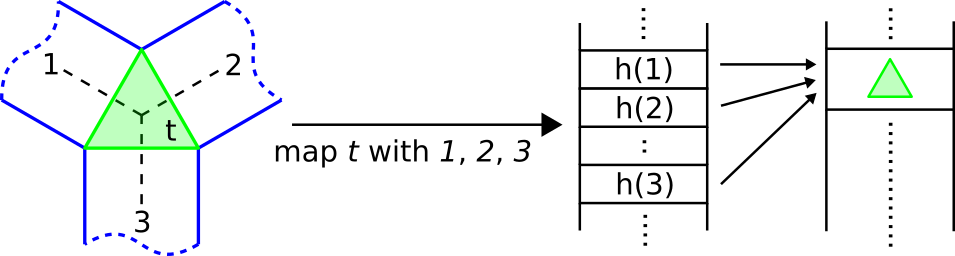
\includegraphics[width=3.3in]{image/hashing.png}
  \caption{An illustration of the data structure for storing spherical triangles. Triangles $t_1$ and $t_2$ are stored linearly in an array and their incident torus $\tau$ is connected to them using a hash table.}
	\label{fig:hashing}
\end{figure}
This allows us, to ray-cast toroidal patches directly instead of tori.


Ray-casting the sphere is a trivial task; nevertheless, in our case the surface sphere of molecules might be formed by an arbitrary number of spherical patches lying in different surface components. To avoid obvious rendering issues, i.e., distinct coloring, transparency or visibility, we perform ray-casting of each spherical patch separately.
This allows us to visually distinguish between different surface components.

Since the boundaries of a spherical patch are formed by small circle arcs, we apply an odd-even rule for polygons~\cite{shimrat1962algorithm} to test whether a point lies inside the patch. Firstly, we compute intersection points, $P_{front}$ and $P_{back}$, of a given ray with the patch sphere.
Here, we describe the point-patch test for point $P_{front}=P$ only, since the same test is applied to $P_{back}$.
Before we apply the odd-even rule, we choose a point $O$ lying outside the patch.
Then, we test line $OP$, the shortest path on a sphere, for an intersection with each of the arcs delimiting the patch.
The intersection of a line $OP$ with the small circle arc, given by points $AB$, is computed in two steps (Fig.~\ref{fig:outer-point}a):
\begin{enumerate}
  \item Intersections of the circles containing the line and the arc, which can intersect in up to $2$ points.
  \item Intersection points are tested whether they belong to both the segment $OP$ and the arc $AB$.
\end{enumerate}
Finally, if the sum of all intersections, i.e., for all the sides, is even then the point lies inside the patch.

\begin{figure}[htp]
  \centering
  \begin{subfigure}[c]{0.52\columnwidth}
    \centering
    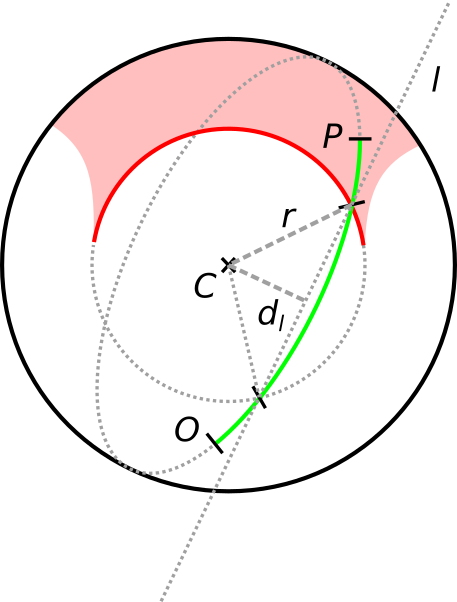
\includegraphics[height=1.9in]{image/patch.png}
    \caption{%Point in spherical patch test.
		The intersection $I_1$ lies on an intersection line between two planes containing arcs $OP$ and $AB$.}
		\label{fig:spherical-patch}
  \end{subfigure}%
  \quad
  \begin{subfigure}[c]{0.44\columnwidth}
    \centering
    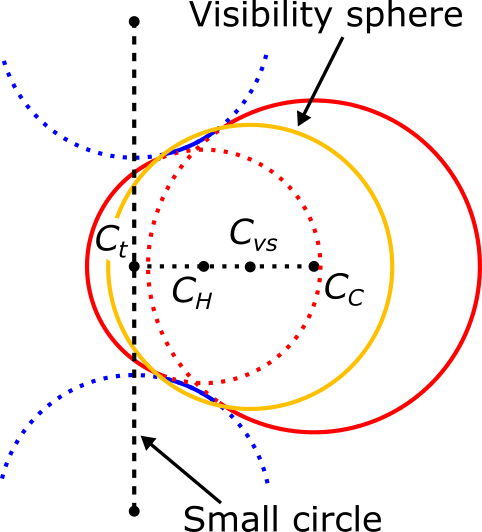
\includegraphics[height=1.6in]{image/outer.png}
    \caption{%A torus formed by carbon ($C_C$) and hydrogen ($C_H$) atoms.
		The center of the torus ($C_{t}$) lies outside the atom centers, while the center of its visibility sphere $C_{vs}$ lies between $C_C$ and $C_H$.}
		\label{fig:outer-point}
  \end{subfigure}
\caption{Point in spherical patch test (a). A torus formed by carbon ($C_C$) and hydrogen ($C_H$) atoms (b).}
\end{figure}

Since we deal with spherical patches and not the planar ones, the situation is bit more complex and we cannot choose point $O$ arbitrarily. 
%Otherwise, we would count intersections of patch's sides with a great circle containing $P$.
%Then, the intersection count would be the same regardless of $P$ being inside or outside the patch, making the rule inapplicable.
Instead, we compute $O$ by intersecting a patch sphere by an axis of one of its delimiting tori.
In this way, we get two intersection points from which we choose the one that lies in the direction of the torus visibility sphere (Fig.~\ref{fig:outer-point}).

%\subsection{Ambient Occlusion Opacity Modulation}
%Borland~\cite{borland2011ambient} proposed to utilize ambient occlusion (AO) values to alter the opacity. Motivated by his approach, we exploit the ambient occlusion values as well. Since, we would like to maintain fast rendering performance, we need to remedy the issue of having an object space technique to evaluate the AO values. In the former work of Borland, the performance was considered a less important factor, which allows him to exploit the full object space AO evaluation. Here, we opted for the most recent approach, proposed by Grottel et al.~\cite{grottel2012object}, which renders ambient occlusion values to a $3D$ grid containing an estimate of the volume area of atoms located inside a voxel. Although this approach only reflects the volume of atoms and not the volume area of the molecular surface, we find it as a good trade off between the visual precision and the performance measure. Note, in addition, these values are not employed directly, but rather as opacity modulators instead, which defines the opacity as follows:
%\begin{equation}
  %\alpha = \left( \frac{O}{\tau}\right)^\rho,
	%\label{eq:alpha}
%\end{equation}
%where $\tau$ represents a threshold such that $alpha=1$ if $O\geq\tau$. Moreover, the resulting $\alpha$ values are clampled to interval $[0,1]$. An example of comparison between different $\tau$ values is depicted in Figure~\ref{fig:TODO}.
%
%Another property we propose to use as the opacity modulator is the surface area of the cavity (TODO do we use this as well, or just using colors?).
%\begin{figure}[htb]
%\centering
  %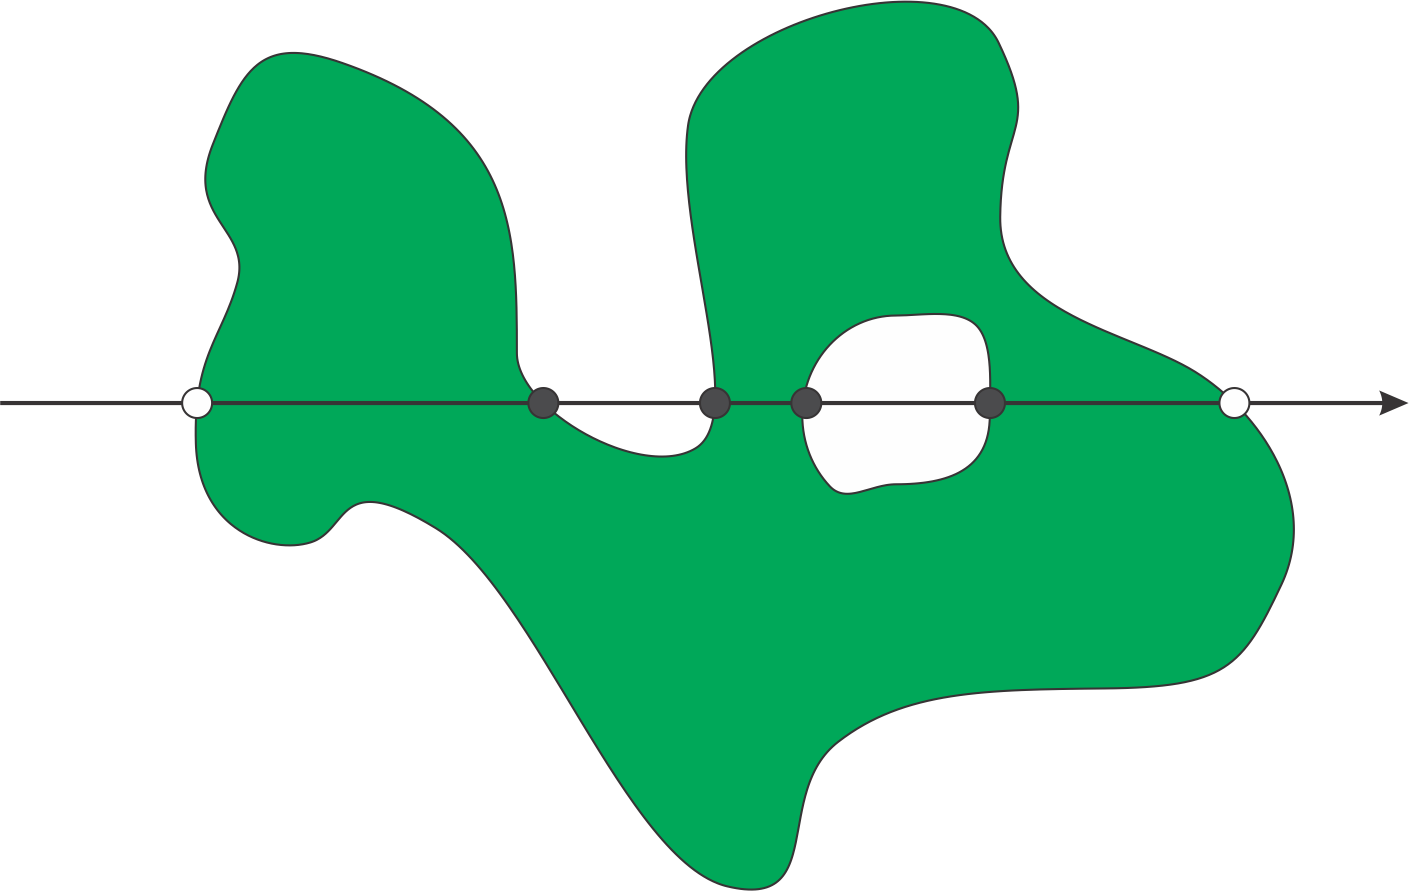
\includegraphics[width=0.8\columnwidth]{image/ray_fragments.png}
  %\caption{(TODO make more nice with overlay AO grid). An example of the list of fragments per a given ray. The color of the circles represent the obtain ambient occlusion value.}
	%\label{fig:ray_fragments}
%\end{figure}

\subsection{Opacity modulation}
After the intersection points were computed, we sort, in front-to-back manner, and store them in the linked list. Thus, for a given ray, we acquire a list of fragments $\{f_1,\ldots,f_n \}$, where each pair represents an entry and an exit point for the molecular surface. For simplicity, the values of $f$ represent depths of fragments. We denote the entire distance the ray passes through the molecule as $l=|f_1-f_n|$. 
As we step along each fragment $f_i$, we define the opacity $\alpha_i$ of even fragments, i.e., those representing the entry surface points, as follows:
\begin{equation}
  \alpha_i = O^{\phi(x)},
	\label{eq:alphaDistEven}
\end{equation}	
where $O$ represents a user defined parameter affecting the overall opacity and $\phi(x)$ suppress or amplifies the opacity and is defined as
\begin{equation}
  \phi(x) = K-(K-1)x,
	\label{eq:exponent}
\end{equation}	
where $K$ is the maximum value of the exponent and $x=|f_{i+1}-f_i|/l$ represents the ratio of the fragment interval to the entire length $l$. Note that if $x=1$, i.e., having just two fragments on the ray, then $\phi(x)=1$ determining the $\alpha_i=O$. The opacity of odd fragments, i.e., representing the exist surface points, is defined as
\begin{equation}
  \alpha_i = O^{L},
	\label{eq:alphaDistOdd}
\end{equation}	
where $L$ is a user defined modulator to suppress or enhance the back-faces.
Figure~\ref{fig:Oparam} showcases $4$ different combinations of parameters $K$ and $O$ with the back-face modulator being constantly set to $L=1$.
\begin{figure*}[htb]
  \centering
  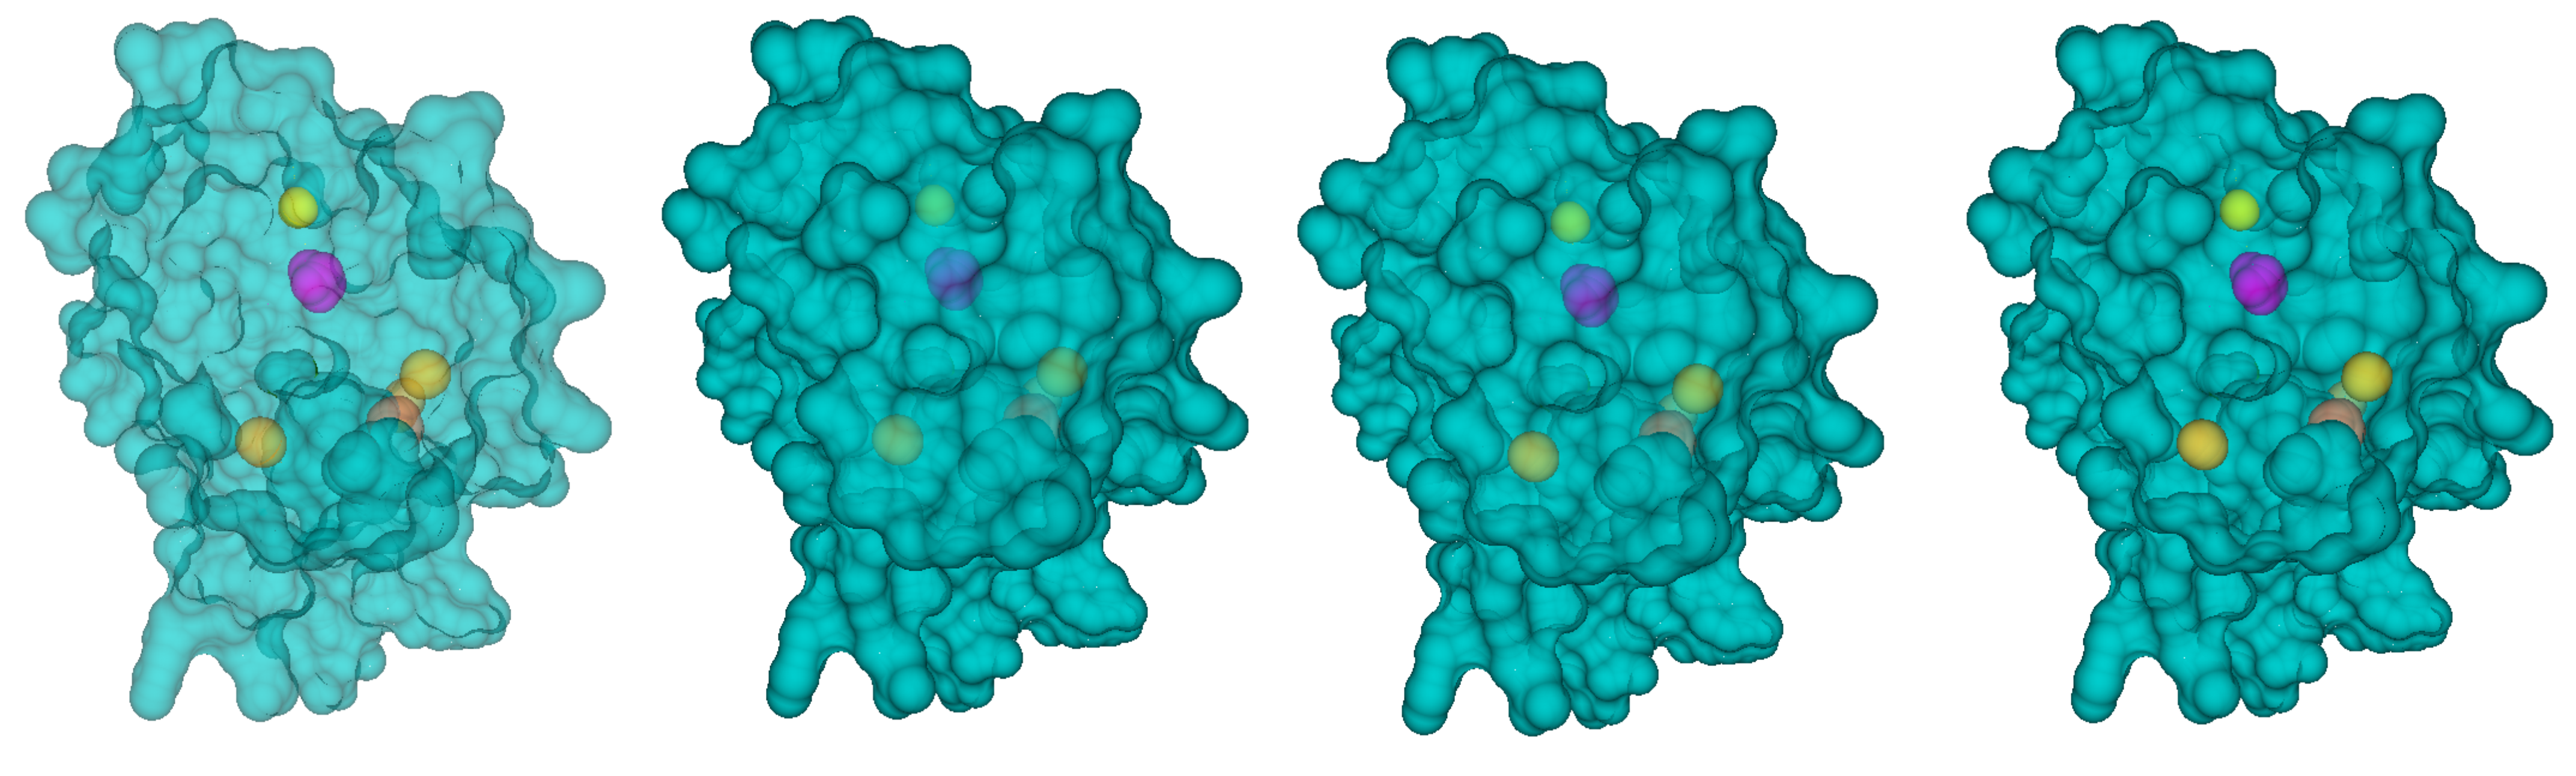
\includegraphics[width=\textwidth]{image/Oparam.png}
  \caption{An example of application of parameters $K$ and $O$ on protein $1cqw$. Note that higher values of the overall opacity $O$ emphasize the front molecular surface, while higher values of maximum exponent $K$ give more prominence to the internal surfaces and cavities.}
	\label{fig:Oparam}
\end{figure*}
\subsection{Cavity area estimation}
We enhance the visualization of cavities by coloring their surface by their approximate areas.
To estimate the area, we sum areas of all triangles that form the cavity surface.
The area of a spherical triangle is calculated as follows:

\begin{equation}
  S = r_{probe}^2 \left[ \left( A + B + C \right) - \pi \right],
\end{equation}

where $A$, $B$ and $C$ are angles of the triangle. 
%We do the area computation in a GLSL compute shader which computes areas of individual triangles and sums them using atomics.
Additionally, we neglect areas of spherical and toroidal patches since their influence on the exact cavity area is much smaller compared to triangles.
%Therefore, the cavity area we compute is \textcolor{red}{underestimated -- maybe an equation?}.
Naturally, this observation does not hold for the molecular surface.
%\textcolor{red}{What about coloring?}
